\let\negmedspace\undefined
\let\negthickspace\undefined
\documentclass[journal]{IEEEtran}
\usepackage[a5paper, margin=10mm, onecolumn]{geometry}
\usepackage{tfrupee} % Include tfrupee package

\setlength{\headheight}{1cm} % Set the height of the header box
\setlength{\headsep}{0mm}     % Set the distance between the header box and the top of the text

\usepackage{gvv-book}
\usepackage{gvv}
\usepackage{cite}
\usepackage{amsmath,amssymb,amsfonts,amsthm}
\usepackage{algorithmic}
\usepackage{graphicx}
\usepackage{textcomp}
\usepackage{xcolor}
\usepackage{txfonts}
\usepackage{listings}
\usepackage{enumitem}
\usepackage{mathtools}
\usepackage{gensymb}
\usepackage{comment}
\usepackage[breaklinks=true]{hyperref}
\usepackage{tkz-euclide} 
\usepackage{listings}                                     
\def\inputGnumericTable{}                                 
\usepackage[latin1]{inputenc}                                
\usepackage{color}                                            
\usepackage{array}                                            
\usepackage{longtable}                                       
\usepackage{calc}                                             
\usepackage{multirow}                                         
\usepackage{hhline}                                           
\usepackage{ifthen}                                           
\usepackage{lscape}
\begin{document}

\bibliographystyle{IEEEtran}
\vspace{3cm}

\title{5.8.4}
\author{EE25BTECH11006 - ADUDOTLA SRIVIDYA}
{\let\newpage\relax\maketitle}

\renewcommand{\thefigure}{\theenumi}
\renewcommand{\thetable}{\theenumi}
\setlength{\intextsep}{10pt} % Space between text and floats

\textbf{Question}:\\
Half the perimeter of a rectangular garden, whose length is $4m$ more than its width,
is $36m$. Find the dimensions of the garden.

\textbf{Solution}:\\
\begin{align}
    \text{Perimeter} &= 2(l+b) \\
    \implies l+b &= 18
\end{align}

Also given,
\begin{align}
    l-b = 4
\end{align}

\begin{align}
    \myvec{1 & 1 \\ 1 & -1}\myvec{l \\ b} = \myvec{18 \\ 4}
\end{align}

Let
\begin{align}
    \vec{A} = \myvec{1 & 1 \\ 1 & -1}, \quad \vec{X} = \myvec{l \\ b}, \quad \vec{Y} = \myvec{18 \\ 4}
\end{align}

\begin{align}
    \vec{A}^T \vec{A} = \myvec{1 & 1 \\ 1 & -1}^T \myvec{1 & 1 \\ 1 & -1} 
          = \myvec{2 & 0 \\ 0 & 2} = 2I
\end{align}

Since $\vec{A}^T \vec{A} = 2I$, we have

\begin{align}
    \vec{A}^{-1} = \dfrac{1}{2}\vec{A}^T
\end{align}

\begin{align}
\vec{X}&= \vec{A}^{-1}\vec{Y} \\
       &= \frac{1}{2}\vec{A}^T \vec{Y} \\
       &= \frac{1}{2}\myvec{1 & 1 \\ 1 & -1}\myvec{18 \\ 4} \\
       &= \frac{1}{2}\myvec{22 \\ 14} \\
       &= \myvec{11 \\ 7}
\end{align}

Therefore,
\begin{align}
    l = 11, \quad b = 7
\end{align}

\begin{figure}[H]
\begin{center}
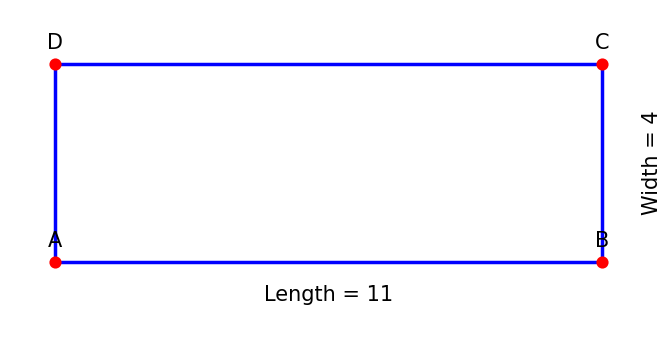
\includegraphics[width=0.7\columnwidth]{figs/fig.png}
\end{center}
\label{fig:Fig1}
\end{figure}

\end{document}